\documentclass[tikz=false]{standalone}
\usepackage[utf8]{inputenc}
\usepackage[dvipsnames,svgnames]{xcolor}
\usepackage{tikz}
\usetikzlibrary{shapes.geometric}
\usetikzlibrary{positioning,graphs, calc}


\begin{document}

  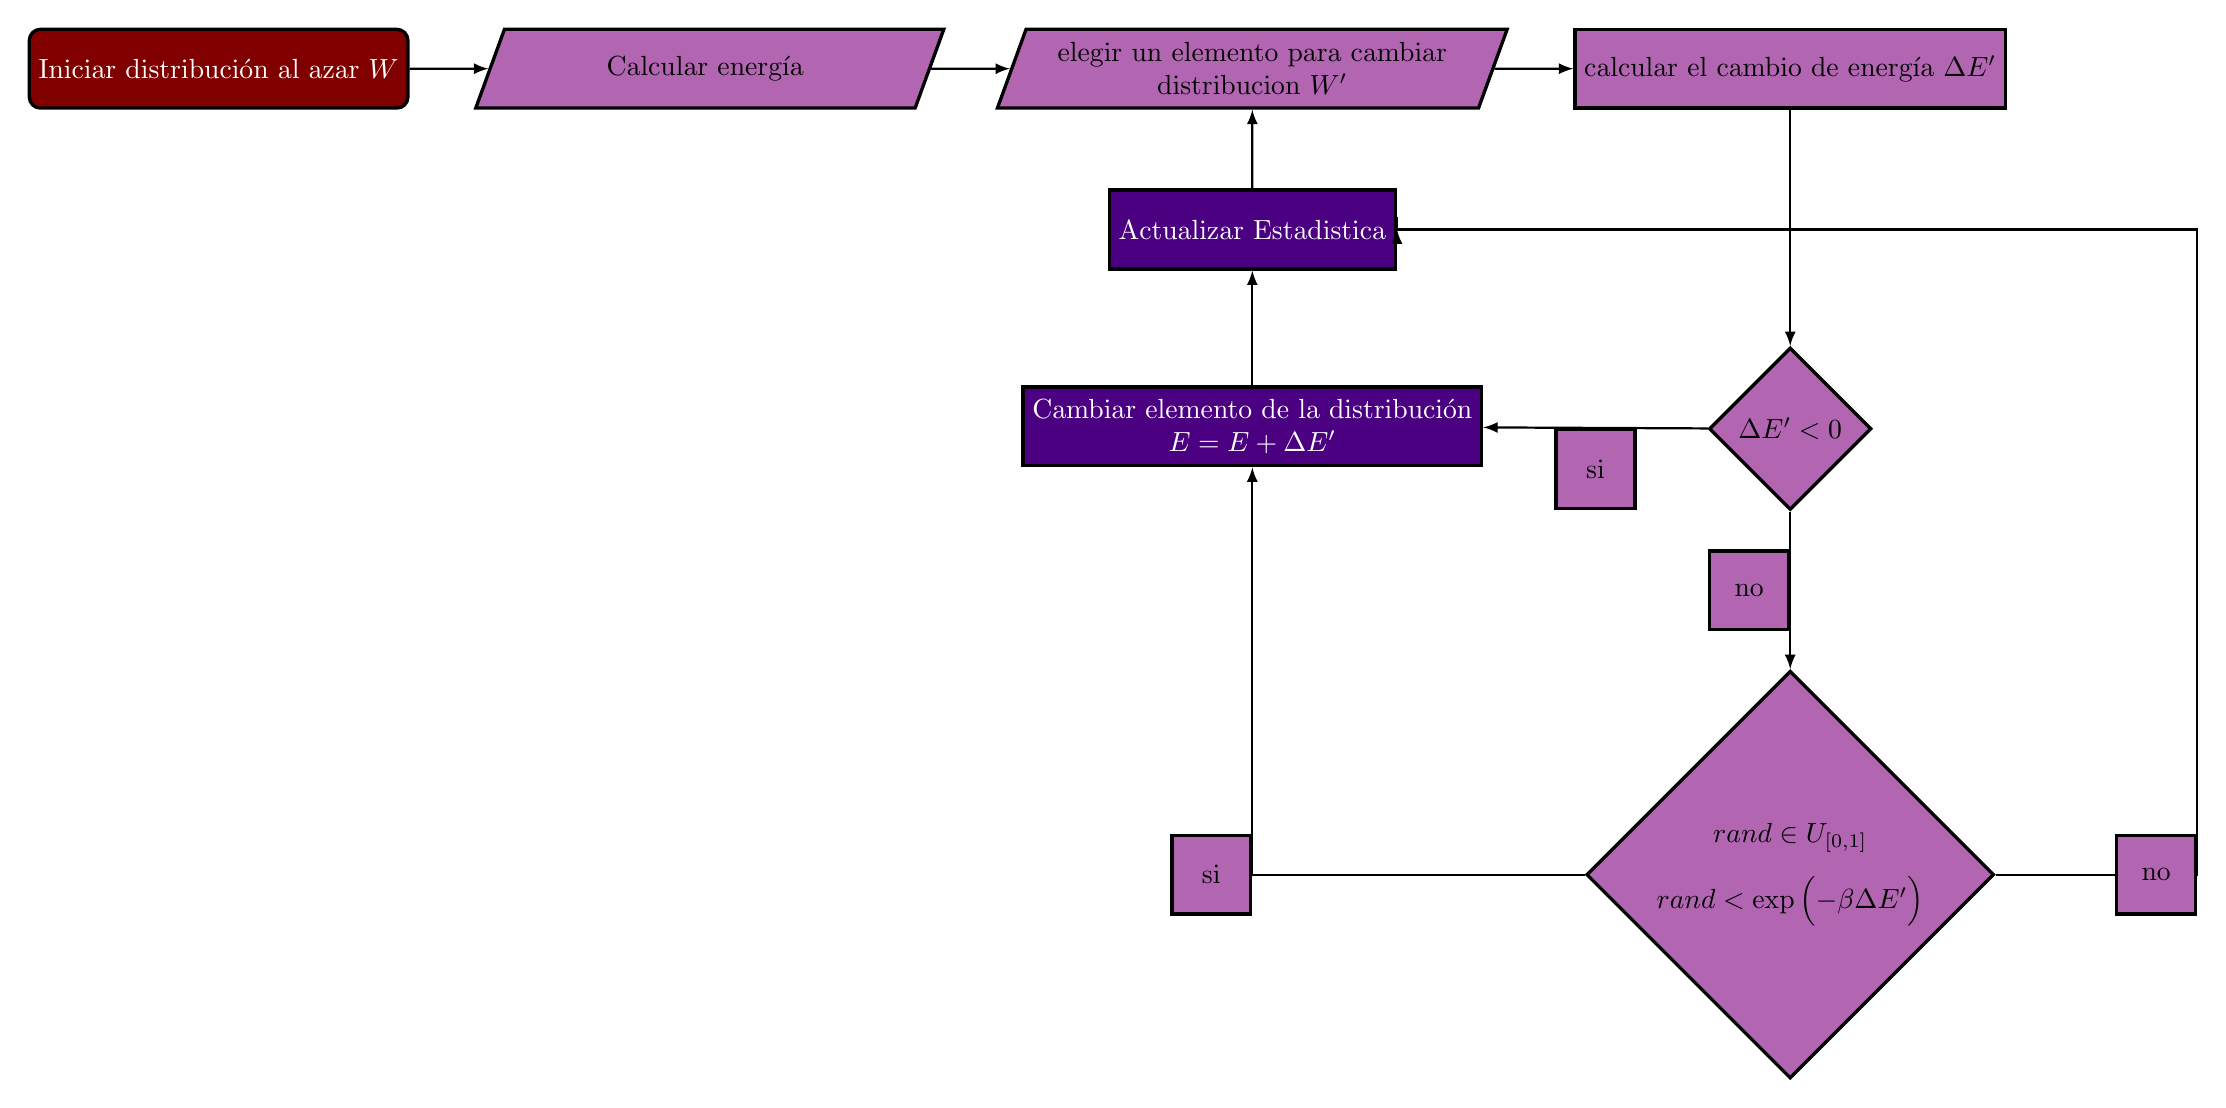
\begin{tikzpicture} [ node distance=1cm,>=latex,auto,
    every node/.style={rectangle, minimum size=1cm, draw, 
    fill=violet!60!white,very thick,align=center} ,
    astep/.style= {trapezium, trapezium left angle=70, trapezium right angle=110},
    start/.style= {
      rectangle, fill=Maroon, rounded corners,text = white
    },
    con/.style={->=stealth,thick },
    decide/.style={diamond,aspect=1},
    action/.style={rectangle, fill=Indigo, text=white}
    ]
    \node (n1) [start] { Iniciar distribución al azar $W$};
    \node (n2) [astep, right=of n1] { Calcular energía };
    \node (n3) [astep, right=of n2 ] { elegir un elemento para cambiar\\
                                            distribucion $W '$ };
    \node (n4) [ right=of n3 ] 
     {calcular el cambio de energía $\Delta E ' $};
        \node (n5) [decide, below =3cm of n4 ] {$\Delta E' < 0 $};
        \node (n6) [decide, below =2cm of n5 ]  
         { $ rand \in U_{[0,1]}$ \\ \\
	   $rand < \exp{\Bigl(-\beta \Delta E'\Bigl)} $};
    \node (n7) [left= 1cm of n5, below =3.5cm of n3, action ]
    { Cambiar elemento de la distribución \\ $E = E + \Delta E'$ };
    \node (n8) [action, above= of n7, below= of n3] {Actualizar Estadistica};

     \draw   [con]  (n1) -- (n2);
     \draw   [con]  (n2) -- (n3);
     \draw   [con]  (n3) -- (n4);
     \draw   [con]  (n4) -- (n5);
     \draw   [con]  (n5) -- node[midway, left]{no} (n6);
     \draw   [con]  (n6) -| node[midway]{si} (n7);  
     \draw   [con] (n5)   -- node[midway]{si} (n7);  
     \draw   [con]  (n7) -- (n8);
     \draw   [con]  (n8) -- (n3);
     \draw   [con]  (n6.east) -|  ($(n6) +(4, 0)$) -|  ($(n8) + (12, 0)$) node[midway]{no} -|  (n8.east);
  \end{tikzpicture}

\end{document}
